\documentclass{article}

\usepackage{graphicx} 
\usepackage[french]{babel}
\usepackage[T1]{fontenc}
\usepackage[utf8]{inputenc}
\usepackage{lmodern}
\usepackage{microtype}
\usepackage{hyperref}
\usepackage{amssymb, amsmath, amsfonts}
\usepackage{geometry}
\usepackage{xcolor}
\usepackage{fancyhdr}
\usepackage{ctex}
\usepackage{tcolorbox}
\pagenumbering{arabic}
\pagestyle{fancy}
\fancyhead[L]{École d'Ingénieurs Paris-SJTU}
\fancyhead[R]{Corentin邱天意}
\fancyfoot[C]{\thepage}
\renewcommand{\headrulewidth}{1pt}
\renewcommand{\footrulewidth}{1pt}

\makeatletter
\@addtoreset{section}{part}
\def\@part[#1]#2{%
    \ifnum \c@secnumdepth >\m@ne
      \refstepcounter{part}%
      \addcontentsline{toc}{part}{\thepart\hspace{1em}#1}%
    \else
      \addcontentsline{toc}{part}{#1}%
    \fi
    {\parindent \z@ \raggedright
     \interlinepenalty \@M
     \normalfont\raggedright
     \ifnum \c@secnumdepth >\m@ne
       \LARGE\bfseries \partname\nobreakspace\thepart
       \par\nobreak
     \fi
     \huge \bfseries #2%
     \markboth{}{}\par}%
    \nobreak
    \vskip 3ex
    \@afterheading}
\renewcommand\partname{Topic}
\makeatother

\title{\textbf{Fiche Sommaire du Cours :\\ FL1902P}}
\author{Corentin邱天意}
\date{Rédigé en Hiver 2025}

\begin{document}

\maketitle

\centerline{
\includegraphics[scale=0.4]{sjtu}}

\newpage

\section*{Avant-propos}
\addcontentsline{toc}{part}{Avant-propos}

FL1902P est le premier cours de mathématiques(et de physique) que les élèves de SPEIT vont rencontrer dans 2,5 ans de classes préparatoires. Plus spécifiquement, toutes les notions et objets mathématiques qu'on va étudier ici font partie des bases des mathématiques. La logique, les ensembles, les méthodes de démonstration et les applications sont à maîtriser si vous souhaitez bien réussir en mathématiques par la suite. Cependant, après avoir entendu les commentaires des professeurs de deuxième année, il est clair que la rédaction et les raisonnements sont encore un désastre. Plus fondamentalement, les élèves ne comprennent pas l'importance de tout cela.

On voit que dans le code du cours, il y a l'abréviation FL pour foreign language, mais cela ne signifie pas qu'on n'y étudiera que la langue. À cause de cela (et du fait que ce cours ne compte que 4 crédits, soit moins qu'un cours de langue, par exemple), certains élèves pensent parfois que c'est un cours facile, sans importance, et qu'il est une perte de temps d'y consacrer trop d'efforts pour bien en comprendre le contenu. Ce sont des opinions erronées et myopes. De plus, il est inutile de blâmer le professeur de mathématiques si quelqu'un n'avait, dès le départ, aucune intention d'apprendre la matière!

Ce fichier servira donc à rappeler les notions fondamentales de FL1902P aux élèves de première ou deuxième année. Il contient quatre chapitres, qui couvrent le programme du cours : la logique, les ensembles, les applications et les démonstrations. J'ai légèrement modifié l'ordre des chapitres, car, pour bien comprendre les ensembles, certains éléments de logique doivent être expliqués au préalable.

Une remarque : le programme de ce cours a été modifié plusieurs fois, et je pense que l'école publiera une version papier plus tard, avec de nombreux changements. Pour ma part, la partie sur les probabilités était encore incluse, mais l'année prochaine, les élèves étudieront la dénombrabilité et la cardinalité, etc. Ici, je ne conserverai que les quatre premiers chapitres.

% Je remercie sincèrement Monsieur Manuel Mansuy pour son cours de MP2I au Lycée Carnot, qui m'ont donné l'idée de comment structurer plusieurs sections, ainsi que plusieurs exercices pour le chapitre sur les démonstrations. Je remercie également l'équipe de mathématiques de l'École SPEIT, surtout Monsieur Hamza (qui est responsable des cours magistraux de FL1902P) et Monsieur Milan (qui a donné ses remarques et retours). Il y aura peut-être les autres à remercier... l'équipe de maths...


Bonne continuation et bon courage à toutes et à tous!


\newpage
\tableofcontents

\newpage



\part{La logique}

Dans cette partie on va rappeler les notions de logique vraiment fondamentales que vous avez vu au lycée ou dans le cours FL1902P. Pas trop difficile mais très important, parce que vous ne pouvez pas construire un bâtiment sans une base, et c'est la base si vous avez envie d'aller plus loin dans les mathématiques de prépa.



\section{Assertions, ensembles, et prédicats}

On définit d'abord les objets mathématiques sans lesquels on ne peut pas progresser. 

\subsection{Assertions}

Pour nous, la notion d'assertion(ou une affirmation) peut être difficile à définir rigoreusement. Cependant, je vais vous donner ici quelques exemples d'affirmations, à partir desquels on peut extraire une définiton généralisée. Voici des exemples:

\begin{itemize}
  \item $1+1=2$
  \item 1 est un entier pair
  \item $x=1$
  \item $ab = ba$
\end{itemize}

La première est vraie, la deuxième est fausse. 3 et 4 sont un peu plus compliquées car leurs vérités dépendent de l'ensemble de définition ou les valeurs de $x$, $a$ et $b$. Par exemple, si on sait déjà que $x$ vaut 1, l'assertion 3 est vraie et fausse sinon; et la 4e est vraie si $a$ et $b$ sont les réels, mais on ne peut rien dire s'ils sont les matrices carrées d'ordre $n$.



Donc, on va utiliser une définition (qui n'est pas vraiment rigoreuse):
\begin{tcolorbox}[colback=red!5!white,colframe=red!75!black,title=Définition 1.1]
  Intuitivement, une \textbf{assertion} est une phrase mathématique sans variable, à laquelle on peut donner un sens. On admet de plus qu'une telle assertion est soit vraie soit fausse.
  \tcblower
  Ici, on dit qu'une assertion est sans variable car les affirmations mathématiques avec variables seront définies plus tard dans ce chapitre(appelées \textbf{Prédicats}).
\end{tcolorbox}

Remarque: dans les exemples que je vous ai donné, le 3 et 4 sont des assertions SEULEMENT si $x$ et $a$, $b$ ont été définies au préalable.

D'une manière similaire, on peut dire(intuitivement) qu'une assertion mathématique ne peut pas être vraie et fausse simultanément. Comme on se place dans le domaine des maths, on a unicité et pas les deux. Plus formellement on dit que c'est le \textbf{principe du tiers exclu}.

Maintenant qu'on a une définition, on pensera immédiatement: Comment puis-je écrire ça d'une manière rigoreuse et claire? Ensuite, comment puis-je écrire moins de mots au cours d'une démonstration? Par convention on peut se donner quelques conseils sur l'écriture. 

Soit $P$ une assertion:
\begin{itemize}
  \item Au lieu de "$P$ est vraie" on écrit souvent "on a $P$" ou "donc $P$"
  \item Au lieu de "supposons que $P$ est une assertion vraie", on écrit "supposons $P$" 
\end{itemize}

\subsection{Ensembles}

Les études axiomatiques et abstraites ne sont pas les destinations pour nous dans cette chapitre, c'est plutôt le vocabulaire et les utilisations que nous nous intéresserons. Vous avez peut-être la question: pourquoi on a une section sur les ensembles dans le chapitre sur la logique? La réponse, c'est que les objets mathématiques sont vraiment liés, et j'ai décidé d'ajouter un petit morceau ici pour qu'on puisse bien faire les quantificateurs après. Voyez le deuxième chapitre sur les ensembles s'ils vous intéressent. 

Voici une définition qui est (encore une fois) informelle:

\begin{tcolorbox}[colback=red!5!white,colframe=red!75!black,title=Définition 1.2]
  Un \textbf{ensemble} est simplement une collection d'objets distincts, et on appelle ces objets "\textbf{éléments}" de l'ensemble.
\end{tcolorbox}

Maintenant qu'on a défini un ensemble et les éléments, on s'intéressera aux notations utilisées.

Soit $E$ un ensemble et $a$ un objet mathématique qui peut appartenir à $E$
\begin{itemize}
  \item Comme on a déjà parlé des assertions, on peut les appliquer ici: L'assertion"$a$ appartient à $E$" ou "l'ensemble $E$ contient $a$" est vraie si $a$ est en fait un élément de $E$, et fausse sinon. On peut utiliser les symboles $\in$ et $\notin$ pour écrire la phrase. 
  \item On utilise habituellement les lettres minuscules pour les éléments et les lettres majuscules pour les ensembles. Mais ce n'est pas toujours le cas(voir la remarque après).
  \item On note l'ensemble $E$ contenant $n$ éléments($a_1$ jusqu'à $a_n$) deux-à-deux distincts: $E=\{a_1, a_2, ... a_n\}$, 
\end{itemize}

Remarque important: Quand on parle des ensembles et des éléments, il faut faire attention: les définitions sont relatives et un objet mathématique peut, à la même fois, être un ensemble et un élément. Tout simplement, un ensemble lui-même peut être un élément d'un autre ensemble, ce qui est parfois difficile à imaginer et comprendre.

\subsection{Prédicats}

\begin{tcolorbox}[colback=red!5!white,colframe=red!75!black,title=Définition 1.3]
  Un \textbf{prédicat} est une phrase mathématique qui fait apparaître des variables, et qui deviendra une assertion vraie ou fausse lorsqu'on y attribue les valeurs.
\end{tcolorbox}

Exemple: voir les exemples que je vous ai donné dans 1.1.1

Remarque: Dans le cas où une assertion dépend d'une variable on peut la noter $P(x)$, avec $x$ la variable et $P$ l'assertion.

\section{Quantificateurs et connecteurs}
\subsection{Quantificateur universel/existentiel}

En fait, idée des quantificateurs est simple: on utilise ces expressions tous les jours à l'oral mais pour qu'on puisse les utiliser dans le langage des maths, on les définit rigoureusement. Il y en a deux qui sont les plus courants et les autres qui sont permutations de ces deux en quelque sort. Comme dans presque tous les exercices, on commence avec les phrases qui décrivent notre situation.

Soit $A(x)$ un prédicat à une variable $x$ qui appartient à l'ensemble $E$. On peut dire que, pour n'importe quelle valeur $x_{0}$ on choisit dans $E$, $A(x_{0})$ soit une assertion. Construisons les explications suivantes:

\begin{tcolorbox}[colback=red!5!white,colframe=red!75!black,title=Définition 1.4]

L'assertion: ``$\forall x \in E, A(x)$'' se lit: ``pour tout $x$ appartenant à $E$, on a A(x)''. Cette assertion est vraie si l'assertion $A(x)$ est vérifiée pour tous les valeurs de $x$ dans $E$.

\tcblower

On appelle le symbole $\forall$ le quantificateur universel.

\end{tcolorbox}

\begin{tcolorbox}[colback=red!5!white,colframe=red!75!black,title=Définition 1.5]

L'assertion: ``$\exists x \in E, A(x)$'' se lit: ``il existe un $x$ appartenant à $E$, tel que $A(x)$''. Cette assertion est vraie s'il existe au moins un $x$ dans $E$ tel que $A(x)$ soit vraie.

\tcblower

On appelle le symbole $\exists$ le quantificateur existentiel.

\end{tcolorbox}

Comprenez bien ces symboles. Quand vous lisez les assertions longs et lourds il faut retenir la logique d'arrière chaque quantificateur. Ne mélangez pas les étapes différents car \c ca peut changer le sens de l'assertion. Vous verrez plein d'exemples plus tard, où les changements d'ordre peut impliquer les définitions très différences(un exemple: la convergence simple et la convergence uniforme for les suites des fonctions que vous allez étudier avec Milan en 2e année).

\subsection{La négation}

Vous avez vu au lycée, qu'avec une assertion il y aura quatre assertions liées qui s'écrivent en utilisant la négation et la contraposition. Ici on va d'abord essayer de définir les connecteurs logiques usuels avant de les utiliser, car au lycée on n' a pas vraiment les étudié d'une manière rigoreuse.

On commence avec la négation, un truc qu'on va très souvent utiliser dans les exercices.

\begin{tcolorbox}[colback=red!5!white,colframe=red!75!black,title=Définition 1.6]

La proposition qui est la ``négation'' ou la ``contraire'' de $P$ est notée $non(P)$. Elle est vraie lorsque $P$ est fausse et fausse lorsque $P$ est vraie.

\end{tcolorbox}

Exemple: les deux assertions suivantes sont les assertions contraires.
\begin{itemize}
 \item $\forall x \in E$, $P(x)$
 \item $\exists x \in E$, $P(x)$ est fausse
\end{itemize}

Ceci est logique, parce qu'on ne peut pas dire qu'un truc marche tous le temps s'il y a les exceptions.

Une remarque: vous avez peut-être vu les exercices qui vous demandent une assertion contraire. Normalement c'est assez facile mais je vous donne un point méthode si vous vous êtes trompé(e)s.

\begin{tcolorbox}[colback=green!5!white,colframe=green!75!black,title=Point méthode 1.1]

Si on veut la négation d'une assertion, on permute les symboles $\forall$ et $\exists$, et puis on nie la conclusion.

\end{tcolorbox}

\subsection{La conjonction et la disjonction}

Je utilise ici les gros mots ``conjonction et disjonction'', mais il existe une manière simple pour décrire qu'est-ce que c'est.

Soit $P$ et $Q$ deux assertions:

\begin{tcolorbox}[colback=red!5!white,colframe=red!75!black,title=Définition 1.7]

\begin{itemize}
 \item La proposition ($P$ \textbf{et} $Q$) est appelée la \textbf{conjonction} des deux assertions. Elle est vraie lorsque $P$ et $Q$ sont toutes les deux vraies, et fausse sinon.
 \item La proposition ($P$ \textbf{ou} $Q$) est appelée la \textbf{disjonction} des deux assertions. Elle est vraie lorsque au moins une des deux assertions sont vraie(s), et fausse sinon.
\end{itemize}

\end{tcolorbox}

\subsection{L'implication}

On écrit toujours les phrases qui sont de la forme: ``si ... alors...'' ou ``on sait que ... donc ...'', et dans les mathématiques on doit expliquer rigoureusement les implications des assertions.

 \begin{tcolorbox}[colback=red!5!white,colframe=red!75!black,title=Définition 1.8.1]

On se donne deux propositions logiques $P$ et $Q$. 

On dit que $P$ implique $Q$ et on note $P \Rightarrow Q$ lorsque, si $P$ est vraie, alors $Q$ est vraie.


\end{tcolorbox}

Point vocabulaire: Si par définition on trouve que $P \Rightarrow Q$, alors on dit que $P$ est une condition suffisante de $Q$ et que $Q$ est une condition
nécessaire de $P$. Pour que $Q$ soit vraie, il suffit que $P$ soit vraie. Pour que $P$ soit vraie, il faut que $Q$ soit vraie. Ca peut être difficile à comprendre, mais ne vous inquiétez pas, c'était le cas pour moi aussi.

Mais justement, vous voyez que ce n'est pas vraiment rigoreuse. C'est facile à comprendre bien sûr, mais on peut faire mieux avec les connecteurs qu'on a définit avant. Voici l'autre définition de l'implication:

 \begin{tcolorbox}[colback=red!5!white,colframe=red!75!black,title=Définition 1.8.2]

On se donne deux propositions logiques $P$ et $Q$. 

L'assertion $(nonP) ou Q$ se note $P \Rightarrow Q$.


\end{tcolorbox}

Lorsque $P$ est fausse, notre assertion est vraie car $nonP$ est vraie. Si les assertions $P$ et $(nonP) ou Q$ sont vraies, par logique, $Q$ est forcément vraie.

Ici on voit que l'assertion $Q$ peut être fausse même si l'assertion $(nonP) ou Q$ est vraie, ce qui peut paraitre bizarre. Mais réfléchissez un peu: on a l'habitude d'utiliser $\Rightarrow$ au lieu de quelques mots de fran\c cais, mais en fait l'utilisation doit être réservée pour les assertions mathématiques. Vous pouvez imaginer les exemples où c'est possible et \c ca servira à éviter les problèmes comme ceci.

Aussi, on voit que la deuxième définition nous permet d'écrire facilement sa négation, avec le point méthode en vert que je vous ai donné.

 \begin{tcolorbox}[colback=blue!5!white,colframe=blue!75!black,title=Propriété 1.1]

On se donne deux propositions logiques $P$ et $Q$. 

La négation de l'assertion $(nonP) ou Q$ s'écrit $P et (nonQ)$


\end{tcolorbox}


Maintenant on sait qu'est-ce que c'est l'implication, mais ce qu'on ne sait pas encore, c'est la démonstration. Comment démontrer l'implication, comment démontrer une autre proposition à partir d'une implication? Je vous donne quelques points méthodes pour les exercices éventuels.

\begin{tcolorbox}[colback=green!5!white,colframe=green!75!black,title=Point méthode 1.2]

Soient $P$ et $Q$ deux assertions. On veut démontrer que $P$ implique $Q$.

\begin{itemize}
 \item Si on sait que l'assertion $P$ est fausse, il n'y a rien à faire.
 \item Si l'assertion $P$ est vraie, alors on doit démontrer que $Q$ est vraie.
\end{itemize}

\tcblower

Si vous commencez comme \c ca: ``Supposons que $P$ est vraie'' et puis essayer de démontrer que $Q$ est vraie, c'est FAUX. Vous ne pouvez pas supposer directement que $P$ est vraie.

\end{tcolorbox}

De la même manière, on peut déduire les choses à partir d'une implication.

\begin{tcolorbox}[colback=green!5!white,colframe=green!75!black,title=Point méthode 1.3]

Soient $P$ et $Q$ deux assertions. On va supposer dans ce cas que $P \Rightarrow Q$.

\begin{itemize}
 \item Si on sait que l'assertion $P$ est vraie, alors dans ce cas $Q$ est forcément vraie aussi.
 \item Si l'assertion $P$ est fausse, ou on ne sait rien sur la vérité de $P$, alors on ne peut rien dire sur la vérité de $Q$.
\end{itemize}



\end{tcolorbox}

\subsection{Réciproque et contraposée}

Ayant définit l'implication, on peut aller plus loin et expliquer la réciproque et la contraposée (et plus tard, l'équivalence) d'une assertion, qui peut aider dans certaines démonstrations.

\begin{tcolorbox}[colback=red!5!white,colframe=red!75!black,title=Définition 1.9]

On se donne deux propositions logiques $P$ et $Q$. 

\begin{itemize}
 \item L’implication $(non Q) \Rightarrow (non P)$ est appelée la contraposition ou la contraposée de $P \Rightarrow Q$.
 \item L’implication $Q \Rightarrow P$ est appelée l’implication réciproque de $P \Rightarrow Q$.
\end{itemize}
 

 
\end{tcolorbox}

 \begin{tcolorbox}[colback=blue!5!white,colframe=blue!75!black,title=Propriété 1.2.1]

L'assertion $P \Rightarrow Q$ est vraie si et seulement si sa contraposée est vraie.

\tcblower

Démonstration: Manipuler les connecteurs et traduire l'implication en utilisant les symboles. C'est un très bon entraînement. On verra une autre méthode plus tard.


\end{tcolorbox}

\subsection{L'équivalence}

\begin{tcolorbox}[colback=red!5!white,colframe=red!75!black,title=Définition 1.10]

On se donne deux propositions logiques $P$ et $Q$. 

On dit que $P$ et $Q$ sont équivalentes si on a (à la même fois) $P \Rightarrow Q$ et $Q \Rightarrow P$. On note dans ce cas $P \Leftrightarrow Q$



\end{tcolorbox}

On peut l'appeler la \textbf{double implication}, et c'est similaire à la double inclusion qu'on voit avec les ensembles. De plus on utilise la notion de $CNS$, qui est l'abréviation de \textbf{condition nécessaire et suffisante} et pas celle de Cell, Nature et Science.

Il reste un point sur lequel on va préciser. C'est effectivement un point méthode: \textbf{la table de vérité}. Elle est notamment utile dans les démonstrations concernant les propositions, et si deux propositions ont même table de vérité, on peut dire qu'elles sont équivalentes. Pour l'écrire, on associe simplement les propositions en colonnes et les différents cas en lignes, ce qui donne un truc comme le figure 1. 

\begin{figure}[!htbp]
 \centering
 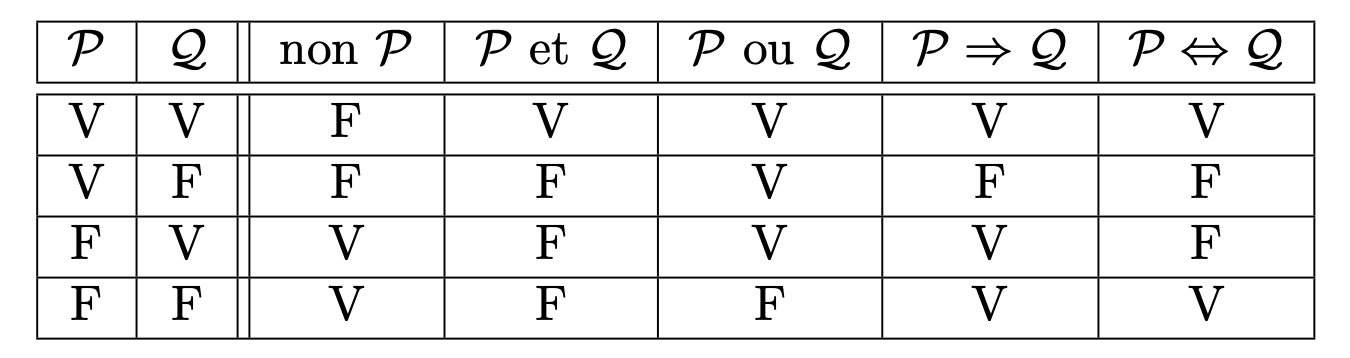
\includegraphics[width=10cm]{tabledeverite.png}
 \caption{Une table de vérité}
\end{figure}

Comme on a définit l'équivalence et donné la méthode de la table de vérité, on peut écrire plus rigoureusement la propriété 1.2 qu'on a vu en utilisant ces notions.

 \begin{tcolorbox}[colback=blue!5!white,colframe=blue!75!black,title=Propriété 1.2.2]

On se donne deux propositions logiques $P$ et $Q$. 

On a: $(P \Rightarrow Q)$ $\Leftrightarrow$ $(nonQ \Rightarrow nonP)$, elles sont équivalentes.

\tcblower

Démonstration: Ecrire les tables de vérité de ces deux propositions.

\end{tcolorbox}

Finalement, révisez bien les exemples et les exercices de TD que Hamza va vous donner(ou vous a donné), ce sont les choses très importantes et vous devez vous entraîner sur cette section des maths.

\newpage
\part{Les ensembles}

On a déjà définit l'ensemble dans la section 1.1.2, et dans ce chapitre on s'intéressera des opérations, les notions novelles et les calculs. On va commencer avec quelques définitions sur les relations entre ensembles. Parmi tous les notions, l'idée de l'inclusion et de l'égalité est la plus simple qui est nécessaire pour qu'on puisse avancer.

Remarque: dans ce chapitre on va rester dans la situation de deux ensembles. Ces notions des relations se généraliseront avec plusieurs ensembles, après la définition de la fonction d'indexation, dans le chapitre suivant. 

\section{Inclusion et égalité}

\subsection{L'inclusion}

En fait cette idée est naturel. Si on a deux sacs qui peut contenir les objets, alors on peut mettre un (petit)sac dans un autre (grand)sac. Dans ce cas, un objet qui se trouve dans le petit sac est aussi dans l'un qui est grand. A partir de cette imagination on peut définit la \textbf{relation d'inclusion} des ensembles.

\begin{tcolorbox}[colback=red!5!white,colframe=red!75!black,title=Définition 2.0]

Regardez la définition d'un ensemble sur la page 5.

\end{tcolorbox}



\begin{tcolorbox}[colback=red!5!white,colframe=red!75!black,title=Définition 2.1]

Soient $E$ et $F$ deux ensembles. 

L'assertion: $\forall x \in F, x \in E$ (qui peut être vraie ou fausse) est noté $F \subset E$, et on dit:``$F$ est une partie de $E$'' ou ``$F$ est inclus dans $E$''

\tcblower

Si l'assertion est vraie on peut dire que $F$ est un \textbf{sous-ensemble} de $F$.


\end{tcolorbox}


Remarque: vous pouvez voir qu'on a enlevé la variable $x$ ici, parce qu'il n'est pas nécessaire pour exprimer une inclusion. C'est une variable \textbf{muette}, à laquelle on peut donner n'importe quel nom.

Alors, pour démontrer cela, on va toujours essayer au début d'utiliser la définiton. Voici un point méthode:

\begin{tcolorbox}[colback=green!5!white,colframe=green!75!black,title=Point méthode 2.1]

Soient $E$ et $F$ deux ensembles. On veut montrer que $F$ est une partie de $E$. Dans ce cas, on prends un élément aléatoire de $F$, et on montre qu'il est aussi un élément de $E$.

Donc il faut commencer avec: ``Soit $x \in F$ ''

\end{tcolorbox}

Avec le point méthode fait ci-dessus on peut démontrer une autre propriété intéressant: le fait que l'inclusion peut être ``transmise'', en quelque sorte.

 \begin{tcolorbox}[colback=blue!5!white,colframe=blue!75!black,title=Propriété 2.1]

Soient $E$, $F$, $G$ trois ensembles. Si $E \subset F$ et $F \subset G$, alors $E \subset G$.

\tcblower

Démonstration: faire en utilisant le point méthode, en s'aidant avec un diagramme si besoin.
\end{tcolorbox} 




Parmi une grande variété d'ensembles, il y en a un qui nous intéresse au début: qu'est-ce qui se passe si on a un ``sac'' vide, avec aucun élément y appartenant? Un tel ensemble peut être vu comme quoi par rapport aux autres ensembles? Formellement on l'appelle \textbf{l'ensemble vide}. Formalisons l'idée:

 \begin{tcolorbox}[colback=blue!5!white,colframe=blue!75!black,title=Propriété 2.2]

Soit $E$ un ensemble et $\emptyset$ l'ensemble vide. $\emptyset \subset E$

\end{tcolorbox} 

\subsection{L'équivalence}


La relation entre ensembles n'est pas un one-way street. On peut imaginer que, si deux ensembles sont exactement les mêmes, alors si je trouve un truc particulier dans le premier, alors le même objet doit exister dans l'autre aussi. En généralisant on obtient la définition de deux ensembles égaux:


\begin{tcolorbox}[colback=red!5!white,colframe=red!75!black,title=Définition 2.2]

Soient $E$ et $F$ deux ensembles. 

Les deux ensembles sont égaux si on a $F \subset E$ et $E \subset F$ à la même fois. Dans ce cas on note $E = F$.


\end{tcolorbox}




\section{Intersection, réunion, différence et complémentaire}

Vous avez certainement vu qu'au lycée on utilise les \textbf{diagrammes de Venn} pour présenter la relation entre ensembles. Si vous essayez de mettre les ensembles sur un plan vous trouverez qu'il y aura les formes qu'on ne sait pas encore décrire. Dans cette section on explique quelques opérations et leurs résultats(qui sont souvent les ensembles aussi).

Remarque: les noms de ces opérations vous donnent déjà quelques idées sur leurs natures. Donc je ne vais pas faire une introduction détaillée pour chaque définition, on se donnera les définitions directement pour gagner du temps.

Note: ajoute les dessins plus tard

\subsection{L'intersection et la réunion}


\begin{tcolorbox}[colback=red!5!white,colframe=red!75!black,title=Définition 2.3]

Soient $E$ et $F$ deux ensembles et $x$ un objet mathématique. 

\textbf{L'intersection} de $E$ et $F$ est notée $E \cap F$ (qui se lit $E$ \textbf{inter} $F$).

On dit que $x$ est un élément de $E \cap F$ s'il appartient à $E$ \textbf{et} à $F$.

\end{tcolorbox}

\begin{tcolorbox}[colback=red!5!white,colframe=red!75!black,title=Définition 2.4]

Soient $E$ et $F$ deux ensembles et $x$ un objet mathématique. 

La \textbf{réunion} de $E$ et $F$ est notée $E \cup F$ (qui se lit $E$ \textbf{union} $F$).

On dit que $x$ est un élément de $E \cup F$ s'il appartient à $E$ \textbf{ou} à $F$.

\end{tcolorbox}

Remarque: Les noms usuels sont assez faciles à retenir. On prend une partie du mot de l'opération.



\subsection{La différence et le complémentaire}

\begin{tcolorbox}[colback=red!5!white,colframe=red!75!black,title=Définition 2.5]

Soient $E$ et $F$ deux ensembles et $x$ un objet mathématique. 

La \textbf{différence} $E - F$ est notée $E \backslash F$ (qui se lit $E$ \textbf{privé de} $F$).

$x$ est un élément de $E \backslash F$ s'il appartient à $E$ mais pas à $F$.


\end{tcolorbox}


\begin{tcolorbox}[colback=red!5!white,colframe=red!75!black,title=Définition 2.6]

Soient $E$ et $F$ deux ensembles et $x$ un objet mathématique. 

Supposons que $F \subset E$, dans ce cas la différence $E \backslash F$ s'appelle le \textbf{complémentaire} de $F$ dans $E$, et on le note $C_{E} F$.



\end{tcolorbox}

Remarque: toutes ces définitions s'écrivent aussi avec la logique propositionnelle.

\section{Ensemble des sous-ensembles}

\begin{tcolorbox}[colback=red!5!white,colframe=red!75!black,title=Définition 2.7]

Soit $E$ un ensemble. 

Il existe l'ensemble des sous-ensembles d'un ensemble, on le note $\mathcal{P}(E)$. 

On a $A \in \mathcal{P}(E) \iff A \subset E$

\tcblower

L'existence est assuré par un axiome de la théorie des ensembles.

\end{tcolorbox}

Cela peut être difficile à comprendre au début. Ici, tous les sous-ensembles de $E$ sont des éléments d'un grand ensemble, qui est l'ensemble des parties de $E$. Attention au fait que les ensembles lui-mêmes peuvent être les éléments.

Exercice: Posons l'ensemble: $E = \{ 1, 2, 3\}$, écrivez l'ensemble $\mathcal{P}(E)$ associé à $E$. Ici, il faut faire attention: l'ensemble $\{1\}$ n'est pas l'élément 1 ou le nombre 1! Pour que deux objets soient égaux il faut qu'ils soient de même nature. C'est similaire à la homogénéité qu'on a vu en physique, avec les unités. 

\section{Couple, n-uplet et produit cartésien}

\subsection{Couples et n-uplets}

Au lycée on a l'habitude de représenter un point sur le plan avec deux variables mises en parenthèses. Par exemple, $(x,y)$ est un point sur le plan $\mathbb{R}^{2}$. On appelle cela un \textbf{couple}.

 \begin{tcolorbox}[colback=blue!5!white,colframe=blue!75!black,title=Propriété 2.3]

Soient $(x_{1},y_{1})$ et $(x_{2},y_{2})$ deux couples dans $\mathbb{R}^{2}$, c'est-à-dire les variables sont des réels.

On a les propriétés suivantes:
\begin{itemize}
 \item $(x_{1},y_{1})$ + $(x_{2},y_{2})$ = $(x_{1} + x_{2}, y_{1} + y_{2})$
 \item Si $(x_{1},y_{1})$ = $(x_{2},y_{2})$, alors $x_{1}$ = $x_{2}$ et $y_{1}$ = $y_{2}$
\end{itemize}

\end{tcolorbox} 

Remarque: 
\begin{itemize}
 \item Cette partie est nécessaire si on veut s'intéresser à la géométrie euclidienne plus tard dans MATH1301P.
 \item Plus généralement on peut construire les ``couples'' avec 3, 4 variables et éventuellement un ``couple'' indexé dans un ensemble. On appelle \textbf{n-uplet} un tel objet avec $n$ variables, ou $n$ est un nombre naturel supérieur à 2.
\end{itemize}

\subsection{Produit cartésien}

Pour qu'on puisse construire les couples(et éventuellement les n-uplets), on définit le \textbf{produit cartésien} de deux ensembles:

\begin{tcolorbox}[colback=red!5!white,colframe=red!75!black,title=Définition 2.8]

Soient $E$ et $F$ deux ensembles. 

On appelle l'ensemble $E \times F$ le \textbf{produit cartésien} de $E$ et $F$, l'ensemble des couples $(x,y)$ avec $x \in E$ et $y \in F$.

On écrit souvent: $E \times F$ = $\{ (x,y); x \in E$ et $y \in F\}$
\tcblower

Cela se généralise avec les n-uplets aussi. 
\end{tcolorbox}

Remarque: On utilise couramment un produit cartésien quand on travaille dans le plan usuel et dans un repère cartésien(voir le cours PHY1301P: Mécanique I) et on identifie chaque point du plan avec le couple de ses coordonnées.






\newpage
\part{Les applications}

Les applications ou les fonctions sont les objets mathématiques très importants, qui apparaissent dans presque tous les sous-domaines. Ici on fait et on explique d'abord l'idée générale des applications, et vous verrez les fonctions réelles plus tard dans MATH1301P.

Dans ce chapitre, on utilisera les notations $E$, $F$, $G$, $H$ pour les ensembles quelconques sans les préciser dans chaque case.


\section{Premières définitions}
\subsection{Définitions}

Une application peut être vue comme une relation entre deux ensembles. Prenons un élément $x$ de $E$, en passant par une application on peut lui associer un élément de $F$(on note souvent $y$). Les opérations mathématiques et physiques passent souvent par une telle applications.

Donc, on va définir chaque objet ($x, y, E, F...$) et quelques notations pour les représenter.

\begin{tcolorbox}[colback=red!5!white,colframe=red!75!black,title=Définition 3.1]

On dit que $f$ est une \textbf{application} de $E$ dans $F$ si, à tout élément $x$ de $E$, $f$ associe un unique élément de $F$, qui est appelé \textbf{l'image} de $x$ par $f$, noté $f(x)$.

$E$ est appelé \textbf{l'ensemble de départ}, et $F$ \textbf{l'ensemble d'arrivée}.

Pour un élément $y$ de l'ensemble $F$, on appelle tout élément $x$ dans $E$ un \textbf{antécédent} de $y$ s'il vérifie $y=f(x)$.


\end{tcolorbox}

Remarque: Observez qu'ici j'ai utilisé les mots ``l'image'' et ``un antécédent''. Ca veut dire que pour un élément de l'ensemble de départ, il n'y a qu'une image, et pour un élément de l'ensemble d'arrivée, on peut trouver plusieurs antécédents. le nombre exact dépend de l'application étudiée et le point choisi.

De plus, deux applications sont \textbf{égaux} si elles ont mêmes ensembles de départ et d'arrivée, et si pour n'importe quel élément dans l'ensemble de départ, ses images par rapport aux deux applications sont égales.

\begin{tcolorbox}[colback=yellow!5!white,colframe=yellow!75!black,title=Notation 3.1]

Avec les variables utilisées dans la définition 3.1, on donne la notation usuelle qui précise toutes les informations.

\[
f : 
\begin{cases} 
E \to F \\
x \mapsto f(x)
\end{cases}
\]

\end{tcolorbox}

Souvent, quand on travaille avec les fonctions on dessine son \textbf{graphe} sur le plan $\mathbb{R}^{2}$. Ici on généralise avec les applications quelconques.

Si on veut dessiner le graphe, on doit connaître tous les points, qui s'expriment comme un couple(l'élément et son image). Prenons un point, deux points, et éventuellement on aura une forme qui représente l'application. Ce n'est pas toujours possible, car il y a les objets qu'on ne sait pas décrire sur un dessin, mais un tel graphe est toujours généralisable de cette manière:

 \begin{tcolorbox}[colback=red!5!white,colframe=red!75!black,title=Définition 3.2]

Soit une application $f$ de $E$ dans $F$.

On appelle \textbf{graphe} de $f$ le sous-ensemble $\Gamma$ de $E \times F$, où $\Gamma$ est définit par: 

\[
\Gamma = \{(x, f(x)), x \in E\}
\]
\end{tcolorbox}

Exemple: Une courbe que vous pouvez dessiner sur le plan $\mathbb{R}^{2}$ est effectivement un de ses sous-ensembles.

Comme on a définit l'ensemble $\mathcal{P}(E)$ d'un ensemble $E$, on fait la même chose avec les applications entre deux ensembles spécifiques.

\begin{tcolorbox}[colback=yellow!5!white,colframe=yellow!75!black,title=Notation 3.2]

On utilise $\mathcal{F}(A,B)$ pour représenter l'ensemble des applications de $A$ dans $B$.


\end{tcolorbox}


\begin{tcolorbox}[colback=purple!5!white,colframe=purple!75!black,title=Remarque importante]

Remarque sur les applications : si on veut définir rigoureusement une application, on la définit à partir de son graphe, donc comme un sous-ensemble de $E \times F$. 

En fait, $f$ est une application de $E$ vers $F$ si $f$ est un sous-ensemble de $E \times E$ vérifiant :
$\forall x \in E, \exists ! y \in F, (x,y) \in f$.

On choisit de noter "$f(x)=y$" plutot que "$(x,y) \in f$".


\end{tcolorbox}


\subsection{Quelques exemples}

Ici on donne quelques exemples importants qui sont à connaîtres.

\begin{itemize}
 \item \textbf{L'identité}: on appelle \textbf{l'application identité} d'un ensemble $E$ l'application qui à $x$ associe $x$(ici $x$ est un élément de $E$). On la note comme :
 \[
{Id}_{E} : 
\begin{cases} 
E \to E \\
x \mapsto x
\end{cases}
\]
 \item \textbf{L'indicatrice}: Supposons que $E$ est un sous-ensemble de $F$. On définit \textbf{l'application indicatrice} de $E$ comme la suivante:
 \[
{1}_{A} : 
\begin{cases} 
E \to \{0,1\} \\
x \mapsto {1}_{A}(x)
\end{cases}
\]
Où ${1}_{A}(x)$ = 1 si $x \in A$, et 0 sinon. Une remarque: voir aussi le symbole de Kronecker $\delta_{i,j}$, l'idée est similaire. On décide si un critère est satisfait, et puis traduire le résultat comme vrai/faux ou 1/0.
 \item \textbf{L'indexation de $E$}: Soit un ensemble $I$ fini (on utilise souvent l'ensemble $I = \{1,2, ... ,n\}$ car cela nous permet d'utiliser les mots premier deuxième, etc). On appelle \textbf{famille d'éléments de $E$ indexée par $I$} toute application de $I$ dans $E$. On note la famille: $(x_{i})_{i \in I}$.
\end{itemize}

Ce dernier exemple est l'indexation dont on a parlé dans le chapitre 2. On peut généraliser les propriétés des fonctions de cette manière.

\subsection{Bref retour aux ensembles indexés}

Au début du chapitre 2 je vous ai expliqué qu'on peut généraliser les notions sur les ensembles avec une indexation. Voici quelques définitions et propriétés que j'ai généralisé en utilisant l'indexation:

\begin{tcolorbox}[colback=yellow!5!white,colframe=yellow!75!black,title={Notation 3.3: Généralisation de la réunion, de l'intersection et du produit cartésien}]



On utilise la notaion $\bigcup\limits_{i \in I} E_i$ au lieu d'écrire l'ensemble: $E_{1}\cup E_{2}\cup E_{3} ... \cup E_{n}$.



On utilise la notaion $\bigcap\limits_{i \in I} E_i$ au lieu d'écrire l'ensemble: $E_{1}\cap E_{2}\cap E_{3} ... \cap E_{n}$.

On utilise la notaion $\prod\limits_{i \in I} E_i$ au lieu d'écrire l'ensemble: $E_{1}\times E_{2}\times E_{3} ... \times E_{n}$.

\tcblower

Ici $I = \{1,2, ... ,n\}$ pour $n$ ensembles, mais on peut prendre $I$ infini.


\end{tcolorbox}

Vous verrez plein d'exemples de l'indexation plus tard...


\section{Injectivité, surjectivité et bijectivité}

On a dit que pour une application $f$ et un élément $x$ dans son domaine de définition, l'image de $x$ par rapport à $f$ est unique, mais la réciproque n'est pas vraie. Donc il est naturel de se demander: pour un spécifique $y$ appartenant à l'ensemble d'arrivée, on peut trouver combien d'antécédents? Et puis, est-ce que c'est généralisable sur tout l'ensemble d'arrivée? En discutant les situations, on peut généraliser ces pensées et produire trois définitions qui portent sur la nature d'une applicaton.

Dans cette section $f$ désigne une application de $E$ dans $F$. De plus je vais utiliser les fonctions usuelles de $\mathbb{R}$ dans $\mathbb{R}$ comme les exemples pour que vous ayez une idée concrète.

\subsection{L'injectivité}

On se demande: combien d'antécédents peut-on trouver pour $y \in F$? Dans cette situation on divise l'univers en trois parties: pas d'antécédent, un unique antécédent et finalement la situation où on a deux ou plus.

Traitons d'abord le cas où on a 0 ou 1:

\begin{tcolorbox}[colback=red!5!white,colframe=red!75!black,title=Définition 3.3]

On dit que l'application $f$ est \textbf{injective} ou qu'elle est une \textbf{injection} si chaque élément de $F$ admet \textbf{au plus} un antécédent dans $E$.

\tcblower

On dit qu'une application est \textbf{non-injective} si elle ne vérifie pas l'assertion énoncée ci-dessus.

\end{tcolorbox}

Remarque: Notez qu'ici on dit \textbf{au plus}. On y ajoute la possibilité des éléments n'ayant pas d'antécédent, parce que rien nous dit que l'ensemble d'arrivée doit être ``rempli''. Il existe souvent les éléments de $F$ qui n'ont pas d'antécédent par rapport à $f$. Par exemple, on dit que l'application qui à $x$ associe $x^{2}$ est une application de $\mathbb{R}$ dans $\mathbb{R}$, mais il y a clairement les valeurs de $\mathbb{R}$ qui n'ont pas de racine carrée réelle(donc pas d'antécédent).

Plus simplement, l'injectivité nous donne l'unicité de l'antécédent lorsqu'il existe.



\begin{tcolorbox}[colback=green!5!white,colframe=green!75!black,title=Point méthode 3.1]

On veut montrer qu'une application $f$ est injective. Elle est injective si et seulement si:

\[
\forall (x_1, x_2) \in E^2, \quad f(x_1) = f(x_2) \Rightarrow x_1 = x_2.
\]

Donc, on prend deux éléments $x_{1}$ et $x_{2}$ satisfaisant $f(x_1) = f(x_2)$, puis démontrer que dans cette situation $x_1 = x_2$.



\end{tcolorbox}




Ayant traité ce cas, on se demandera de plus: il y a les éléments de l'ensemble d'arrivée qui n'ont pas d'antécédent. Comment décrire ce phénomène? L'ensemble est-il rempli? Pour \c ca on va définir la surjectivité.






\subsection{La surjectivité}

\begin{tcolorbox}[colback=red!5!white,colframe=red!75!black,title=Définition 3.4]

On dit que l'application $f$ est \textbf{surjective} ou qu'elle est une \textbf{surjection} si chaque élément de $F$ admet \textbf{au moins} un antécédent dans $E$.

\tcblower

On dit qu'une application est \textbf{non-surjective} si elle ne vérifie pas l'assertion énoncée ci-dessus.

\end{tcolorbox}


\begin{tcolorbox}[colback=green!5!white,colframe=green!75!black,title=Point méthode 3.2]

On veut montrer qu'une application $f$ est surjective. Elle est surjective si et seulement si:

\[
\forall y \in F, \exists x \in E,  f(x) = y.
\]

Donc, on prend un élément quelconque de $F$ puis démontrer qu'il existe au moins un antécédent.



\end{tcolorbox}

Finalement, si une application est à la fois injective et surjective, alors il y a une correspondance biunivoque(gros mot ici, \c ca veut dire one-to-one en anglais). On donne un nom: la bijectivité.




\subsection{La bijectivité}

\begin{tcolorbox}[colback=red!5!white,colframe=red!75!black,title=Définition 3.5]

On dit que l'application $f$ est \textbf{bijective} ou qu'elle est une \textbf{bijection} si chaque élément de $F$ admet un \textbf{unique} antécédent dans $E$.

\tcblower

On dit qu'une application est \textbf{bijective} si elle est à la fois injective et surjective.
\end{tcolorbox}

C'est une bonne propriété pour une application, car elle nous donne la correspondance biunivoque entre les éléments de deux ensembles. Plus tard vous allez voir que cela peut être lié avec la cardinalité des ensembles. Dans la définiton, le mot "chaque" nous donne la surjectivité, et le mot "unique" nous donne l'injectivité. Il est naturel de conclure que la bijectivité peut être vue comme une combinaison de ces deux.





\section{La composition}
\subsection{Composition des fonctions}
Les transformations peut être faites une après l'autre. Dans les calculs on peut décider de d'abord ajouter 2, puis multiplier par 3, ou bien d'abord multiplier par 3, puis ajouter 2. On peut généraliser cette idée avec les applications, plus spécifiquement la composition.

\begin{tcolorbox}[colback=red!5!white,colframe=red!75!black,title=Définition 3.6]

Soient $f$ une application de $E$ dans $F$ et $g$ une application de $F$ dans $G$.

On appelle \textbf{composition} de $g$ et $f$ l'application notée $g \circ f$ définie par:

\[ g \circ f :
\begin{cases}
E \to G \\ 
x \mapsto g(f(x))
\end{cases}
\]

\end{tcolorbox}

Remarque: attention à l'ordre des opérations! Pour l'application $g \circ f$ on passe d'abord par $f$ et puis par $g$.

Le sens est assez claire pour cette opération. Mais pour qu'elle soit bien définie, on doit vérifier que l'image de $x$ par $f$ est dans le domaine de définition de $g$. Il y a quelques propriétés simples qui peuvent être utilisées en passant par la composition, notamment les trois dont on vient de parler.

\begin{tcolorbox}[colback=blue!5!white,colframe=blue!75!black,title=Propriété 3.1]

Soient $E, F, G, H$ des ensembles et $f \in \mathcal{F}(E,F), g \in \mathcal{F}(F,G), h \in \mathcal{F}(G,H)$.
\begin{itemize}
    \item Pour tout $f \in \mathcal{F}(E,F)$, on a : $f \circ Id_E = f$.
    \item Pour tout $f \in \mathcal{F}(E,F)$, on a : $Id_F \circ f = f$.
    \item La composition est associative : 
    \[
    (h \circ g) \circ f = h \circ (g \circ f).
    \]
\end{itemize}

\end{tcolorbox} 

Remarque: Notez que dans les deux premiers points on a utilisé deux identités différents, car ``au milieu'' des deux applications on doit trouver le même ensemble.

La propriété 3.1 est fondamentale. On continue avec les propriétés résultantes sur l'injectivité, la surjectivité et la bijectivité.


\begin{tcolorbox}[colback=blue!5!white,colframe=blue!75!black,title=Propriété 3.2]

On se donne deux applications $f : E \to F$ et $g : F \to G$.

\begin{itemize}
    \item Si $f$ et $g$ sont injectives, alors $g \circ f$ est injective. \\
    Inversement, si $g \circ f$ est injective, alors $f$ est injective.

    \item Si $f$ et $g$ sont surjectives, alors $g \circ f$ est surjective. \\
    Inversement, si $g \circ f$ est surjective, alors $g$ est surjective.

    \item Si $f$ et $g$ sont bijectives, alors $g \circ f$ est bijective. \\
    Inversement, si $g \circ f$ est bijective, alors $f$ est injective et $g$ est surjective.
\end{itemize}

\end{tcolorbox} 

Prenez du temps et démontrer ces propriétés vous-mêmes, c'est un bon entraînement logique, et sachez que l'intuition n'est pas toujours correcte dans ce domaine car ces trois propriétés ne sont pas évidentes.

\subsection{L'application récoproque}

Ayant parlé de la bijectivité, on peut imaginer que: si une application est bijective, alors pour un élément du domaine de définition, on peut lui associer son image unique. De plus le sens réciproque est vraie: pour l'image on peut trouver un unique antécédent. Cela nous permet de construire \textbf{l'application réciproque} ou \textbf{la bijection réciproque}.

\textbf{Il faut justifier que ce soit une bijection avant de définir sa réciproque!}

\begin{tcolorbox}[colback=red!5!white,colframe=red!75!black,title=Définition 3.7]

Soient $f$ une application de $E$ dans $F$ qui est \textbf{bijective}.

On appelle \textbf{l'application réciproque} de  $f$ l'application notée $f^{-1}$ définie par:

\[ 
f^{-1} :
\begin{cases}
F \to E \\ 
y \mapsto f^{-1}(y)
\end{cases}
\]

Ici $f^{-1}(y)$ est l'unique antécédent de $y$ par $f$, qui existe et est unique grâce à la bijectivité de $f$.

\end{tcolorbox}


A partir de ceci on trouvera quelques propriétés qui sont, encore une fois, liées aux propriétés des applications déjà expliquées.

\begin{tcolorbox}[colback=blue!5!white,colframe=blue!75!black,title=Propriété 3.3]



On se donne deux applications $f : E \to F$ et $g : F \to G$.

\begin{itemize}
    \item Si $f$ et $g$ sont les bijections, alors $g \circ f$ est aussi une bijection. Ces applications et leurs réciproques vérifie la relation: 
    \[
    (g \circ f)^{-1} = f^{-1} \circ g^{-1}.
    \]

    \item Si $f$ est une \textbf{bijection} de $E$ dans $F$, alors son application réciproque $f^{-1}$ est aussi bijective, vérifiant:$(f^{-1})^{-1} = f$.

\end{itemize}



\end{tcolorbox} 


On utilise parfois une autre méthode/propriété pour démontrer qu'une application est bijective, en utilisant la relation avec l'identité.

\begin{tcolorbox}[colback=blue!5!white,colframe=blue!75!black,title=Propriété 3.4]


L'application $f$ de $E$ dans $F$ est \textbf{bijective} si et seulement s’il existe une application $g$ de $F$ dans $E$ telle que :
\[
g \circ f = Id_E \quad \text{et} \quad f \circ g = Id_F.
\]
L’application $g$ est alors \textbf{l'application réciproque} de $f$.


\end{tcolorbox} 


\section{Images directes et réciproques}

Étant donné un élément, on peut lui associer une image. Dans cette section on étend ceci aux ensembles, qui ne sont que les collections d'éléments.

\begin{tcolorbox}[colback=red!5!white,colframe=red!75!black,title=Définition 3.8]

Soit $f \in \mathcal{F}(E,F)$. Si $A \subset E$ et $B \subset F$, on appelle :
\begin{itemize}
    \item \textbf{image directe} de $A$ par $f$, l’ensemble :
    \[
    f(A) = \{ y \in F \mid \exists x \in A \quad y = f(x) \} = \{ f(x) ; x \in A \},
    \]
    \item \textbf{image réciproque} de $B$ par $f$, l’ensemble :
    \[
    f^{-1}(B) = \{ x \in E \mid f(x) \in B \}.
    \]
\end{itemize}
\end{tcolorbox}

Vous pouvez voir que l'image directe d'un ensemble est la collection des images de ses éléments, et l'inverse pour l'image réciproque.

Attention: j'écris $f^{-1}(B)$ pour l'image réciproque de $B$ par $f$, mais $f$ n'est pas forcément bijective, ne confondre pas avec l'application réciproque. 

Vous trouverez qu'une application et ses propriétés sont très générales, car on ne spécifie pas la nature des éléments. Plus tard vous allez étudier d'abord les fonctions réelles des variables réelles, où l'ensemble de définition est une partie de $\mathbb{R}$, et les fonctions vectorielles, qui projète les éléments dans l'espace de dimension $n$. Travaillez bien ce chapitre pour que vous puissiez maîtriser les autres chapitres plus tard.





\newpage
\part{La démonstration}

Dans cette partie on va donner quelques types de raisonnements pour vous aider dans les démonstrations. Après chaque point, vous trouverez un exemple classique ou un exemple extrait du cours/TD de Monsieur Hamza que j'ai suivi, avec la correction, pour vous montrer comment rédiger proprement un exercice.


\section{À partir des définitions...}

Dans cette section on donne les méthodes et les propriétés qui sont utiles pour les démonstrations. Comme le titre dit, la majorité de ces méthodes sont les applications directes des définitions qu'on connaît déjà.

\subsection{Assertions universelles}

On veut montrer une \textbf{assertion universelle}, c'est-à-dire une assertion de la forme générale:

\[
\forall x \in E, P(x)
\]

Où $E$ est un ensemble et $P(x)$ un prédicat dépendant de $x$.

\begin{tcolorbox}[colback=green!5!white,colframe=green!75!black,title=Point méthode 4.1]

Dans ce cas, comme on veut le démontrer pour tous les éléments, on prend un élément $x$ quelconque de $E$, puis démontrer $P(x)$. 

\end{tcolorbox}


\begin{tcolorbox}[colback=cyan!5!white,colframe=cyan!75!black,title=Exercice]

Montrer que: $\forall x \in \mathbb{R}, \frac{x}{x^{2}+1} \leq \frac{1}{2}$

\end{tcolorbox}

\paragraph{Preuve:} On commence toujours par ``\textbf{soit}''

\noindent Preuve à rédiger









\subsection{Assertions existentielles}

On veut montrer une \textbf{assertion existentielle}, c'est-à-dire une assertion de la forme générale:

\[
\exists x \in E, P(x)
\]

Où $E$ est un ensemble et $P(x)$ un prédicat dépendant de $x$.

\begin{tcolorbox}[colback=green!5!white,colframe=green!75!black,title=Point méthode 4.2]

L'existence se démontre avec un exemple, c'est-à-dire on peut démontrer l'assertion en posant un $x$ particulier, avec $P(x)$ vraie.

\end{tcolorbox}


\begin{tcolorbox}[colback=cyan!5!white,colframe=cyan!75!black,title=Exercice]

Montrer que: $\forall (x,y) \in \mathbb{R}^{2}, \exists z \in \mathbb{R}, z > x + y $

\end{tcolorbox}

\paragraph{Preuve:} Avez-vous un \textbf{exemple} à donner?

\noindent Preuve à rédiger











\subsection{Implication(des assertions)}

Je vous rappelle le point méthode 1.2 qu'on a vu dans le premier chapitre.

\begin{tcolorbox}[colback=green!5!white,colframe=green!75!black,title=Point méthode 4.3/1.2]

Soient $P$ et $Q$ deux assertions. On veut démontrer que $P$ implique $Q$.

\begin{itemize}
 \item Si on sait que l'assertion $P$ est fausse, il n'y a rien à faire.
 \item Si l'assertion $P$ est vraie, alors on doit démontrer que $Q$ est vraie.
\end{itemize}

\tcblower

Si vous commencez comme \c ca: ``Supposons que $P$ est vraie'' et puis essayer de démontrer que $Q$ est vraie, c'est FAUX. Vous ne pouvez pas supposer directement que $P$ est vraie. 

Parfois on doit faire une disjonction des cas, la méthode que vous allez voir plus tard.

\end{tcolorbox}

Remarque: Je dis qu'on doit discuter d'abord la vérité de $P$, mais dans les exercices on commence(presque toujours) avec une assertion vraie. Prenez garde quand même.


\begin{tcolorbox}[colback=cyan!5!white,colframe=cyan!75!black,title=Exercice]

Montrer que: $\forall x \in [0,1], x - x^{2} \in \mathbb{N} \Rightarrow x \in \{0,1\} $


\end{tcolorbox}

\paragraph{Preuve:} La vérité de la première assertion implique quoi?

\noindent Preuve à rédiger














\subsection{Équivalence(des assertions)}

Deux assertions $P$ et $Q$ sont équivalentes si et seulement si les assertions $P \Rightarrow Q$ et $Q \Rightarrow P$ sont vraies.

\begin{tcolorbox}[colback=green!5!white,colframe=green!75!black,title=Point méthode 4.4]

Écrivez deux étapes et démontrer l'implication pour chaque étape.

\end{tcolorbox}


\begin{tcolorbox}[colback=cyan!5!white,colframe=cyan!75!black,title=Exercice]

Soit \( x \in \mathbb{R} \). Montrer que : $\sqrt{x+4} - \sqrt{x+2} = 1 \text{ si et seulement si } x = \frac{-7}{4}$


\end{tcolorbox}


\paragraph{Preuve:} Le sens direct et le sens réciproque!

\noindent Preuve à rédiger














\subsection{Inclusion des ensembles}

\begin{tcolorbox}[colback=green!5!white,colframe=green!75!black,title=Point méthode 4.5/2.1]

Soient $E$ et $F$ deux ensembles. On veut montrer que $F$ est une partie de $E$. Dans ce cas, on prends un élément aléatoire de $F$, et on montre qu'il est aussi un élément de $E$.

Donc il faut commencer avec: ``Soit $x \in F$ ''

\end{tcolorbox}


\begin{tcolorbox}[colback=cyan!5!white,colframe=cyan!75!black,title=Exercice]

On note \( 2\mathbb{N} \) l’ensemble des entiers naturels pairs, et on pose :$E = \{k(k+1), k \in \mathbb{N}\}$.
Montrer que : $E \subset 2\mathbb{N}$

\end{tcolorbox}

\paragraph{Preuve:} Commencez avec ``soit''

\noindent Preuve à rédiger
















\subsection{Égalité des ensembles}

\begin{tcolorbox}[colback=green!5!white,colframe=green!75!black,title=Point méthode 4.6]

Deux ensembles sont égaux si on peut démontrer la double inclusion.

\end{tcolorbox}


\begin{tcolorbox}[colback=cyan!5!white,colframe=cyan!75!black,title=Exercice]

Montrer les égalités suivantes :

\[
| -1, 1 | = \bigcup_{n \in \mathbb{N}^*} \left[ -1 + \frac{1}{n}, 1 - \frac{1}{n} \right] \quad \text{et} \quad [-1, 1] = \bigcap_{n \in \mathbb{N}^*} \left[ -1 - \frac{1}{n}, 1 + \frac{1}{n} \right]
\]

\end{tcolorbox}

\paragraph{Preuve:} Encore une fois, deux sens à rédiger

\noindent Preuve à rédiger
















\subsection{Unicité}

On veut montrer que l'objet  $x$ qui vérifie $P(x)$ est unique.

\begin{tcolorbox}[colback=green!5!white,colframe=green!75!black,title=Point méthode 4.7]

Soient \( x, x' \in E \).  
Faisons l'hypothèse que \( \mathcal{P}(x) \) et \( \mathcal{P}(x') \).  
Montrons que : \( x = x'. \) 

\end{tcolorbox}

Remarque: On veut montrer l’unicité d’un objet dans un ensemble \( E \) vérifiant une propriété \( \mathcal{P} \), ceci n’est pas équivalente à montrer l’assertion : \(\exists! x \in E, \, \mathcal{P}(x)\)! Pour une assertion $\exists!$ on doit montrer l'existence et l'unicité, mais c'est le deuxième qu'on veut démontrer ici.



\begin{tcolorbox}[colback=cyan!5!white,colframe=cyan!75!black,title=Exercice]

Soit $E$ un ensemble. 

Montrer que: $\exists ! A \in \mathcal{P}(E), \forall B \in \mathcal{P}(E), A \subset B$.

\end{tcolorbox}


\paragraph{Preuve:} Existence, puis unicité.

\noindent Preuve à rédiger
















\section{Méthodes et types de démonstration}


Cette section donne les ``vraies'' méthodes, et pas simplement celles qui s'obtiennent directement avec les définitions. Vous devez penser à ces méthodes si vous êtes bloqués dans une démonstration.

Remarque: les méthodes non étoilées sont celles qui ont été introduites par Hamza pendant les cours magistraux. J'ai mis des étoiles sur les méthodes qui ne sont pas directement au programme, mais elles peuvent être utiles. Jetez un coup d'oeil si vous voulez.


\subsection{Raisonnement par disjonction des cas*}

Dans un exercice un peu plus compliqué on trouve qu'il y a besoin de discuter plusieurs cas. On commence par écrire les cas possibles, puis on démontre pour chaque cas séparément. C'est une intuition que vous avez déjà rencontré au lycée, et vous savez qu'il est important de ne pas oublier un cas, de ne pas répéter un cas.


\begin{tcolorbox}[colback=green!5!white,colframe=green!75!black,title=Point méthode 4.8]


On se donne un exemple: une assertion universelle. Supposons qu'on veut démontrer l'assertion: $\forall x \in \mathbb{E}, P(x)$. En séparant $E$ comme $E = E_1 \cup E_2 \cup ... \cup E_n$, puis en preuvant $P(x)$ pour chaque $E_i$, on peut montrer l'assertion universelle.

\tcblower

Ici la famille peut être indexée.




\end{tcolorbox}


\begin{tcolorbox}[colback=cyan!5!white,colframe=cyan!75!black,title=Exercice]


\end{tcolorbox}



\subsection{Raisonnement déductif*}

\begin{tcolorbox}[colback=green!5!white,colframe=green!75!black,title=Point méthode 4.9]

Pour montrer qu'une proposition \( Q \) est vraie, il suffit de montrer qu'une proposition \( P \) est vraie et que \( P \Rightarrow Q \).


\end{tcolorbox}

Remarque: Il faut que l'assertion $P$ soit vraie! La vérité de l'implication \( P \Rightarrow Q \) ne signifie pas celle de $Q$!

\begin{tcolorbox}[colback=cyan!5!white,colframe=cyan!75!black,title=Exercice]


\end{tcolorbox}



\subsection{Raisonnement par la contraposée}

Rappelez-vous que la contraposée d'une implication $P \Rightarrow Q$ est $non Q \Rightarrow non P$, et qu'elles ont même valeur de vérité dans une TDV.

\begin{tcolorbox}[colback=green!5!white,colframe=green!75!black,title=Point méthode 4.10]

On peut essayer de démontrer une implication en démontrant sa contraposée, car $P \Rightarrow Q$ est équivalente à $non Q \Rightarrow non P$

\end{tcolorbox}


\begin{tcolorbox}[colback=cyan!5!white,colframe=cyan!75!black,title=Exercice]


\end{tcolorbox}



\subsection{Raisonnement par l'absurde}

C'est une méthode utile si on trouve que l'assertion à démontrer est trop difficile si on essaye dans le sens direct.

\begin{tcolorbox}[colback=green!5!white,colframe=green!75!black,title=Point méthode 4.11]

Pour montrer qu'une proposition $P$ est vraie, on peut montrer que \(nonP \Rightarrow \textbf{Faux}\). On écrira ainsi :

\begin{itemize}
    \item \textbf{Supposons \(P\) fausse}
    \begin{itemize}
        \item \dots
        \item \(\downarrow\) Une contradiction! Ou un truc qui est clairement faux.
        \item Par conséquent, \(P\) est vraie.
    \end{itemize}
\end{itemize}


\end{tcolorbox}

Remarque: C'est effectivement la combinaison de 2.2 et de 2.3. Pour commencer, \(nonP \Rightarrow \textbf{Faux}\) est(par sa contraposition) équivalente à \(\textbf{Vrai} \Rightarrow P\). En utilisant un raisonnement déductif et un truc qui est vrai, on montre que $P$ est vraie.




\begin{tcolorbox}[colback=cyan!5!white,colframe=cyan!75!black,title=Exercice]


\end{tcolorbox}





\subsection{Raisonnement par analyse-synthèse}

On considère un prédicat \( P(x) \) dépendant d'une variable \( x \in E \). On souhaite déterminer l'ensemble des solutions associé à \( P \), c'est-à-dire l'ensemble \( S \) des \( x \) dans \( E \) tels que \( P(x) \) est vraie.


\begin{tcolorbox}[colback=green!5!white,colframe=green!75!black,title=Point méthode 4.12]

Pour déterminer l'ensemble des \( x \) dans \( E \) tels que \( P(x) \) est vraie, il peut être intéressant de procéder par \textbf{Analyse - Synthèse}. Le raisonnement se fait en deux temps :

\begin{itemize}
    \item \textbf{Analyse.} On fixe \( x \in E \).
    
    On suppose que \( P(x) \) est vraie, et on en déduit des conditions nécessaires sur \( x \).
    
    On restreint ainsi le champ des solutions possibles à un sous-ensemble \( C \) de \( E \) qui satisfait \( S \subset C \).
    
    \item \textbf{Synthèse.} Pour chaque élément \( x \in C \) satisfaisant les conditions nécessaires de l'analyse, on vérifie si \( P(x) \) est vraie ou fausse, et donc si \( x \in S \) ou \( x \notin S \). On détermine ainsi si les conditions obtenues sont suffisantes ou non.
\end{itemize}

À l'issue de ces deux étapes, on obtient l'ensemble \( S \) des éléments de \( E \) qui satisfont la propriété \( P \).



\end{tcolorbox}


Remarque: Le raisonnement par Analyse - Synthèse est souvent employé pour montrer les propositions de la forme « \( \exists!x \in E \), \( P(x) \) ». Dans ce cadre, l'analyse réduit le champ des solutions possibles jusqu'à l'obtention d'un unique élément \( x \in E \), puis la synthèse vérifie que cet élément est bel et bien solution.

L'avantage de passer par un raisonnement par Analyse - Synthèse est qu'il est difficile sinon de « deviner » un élément \( x \) solution du problème. En montrant l'unicité dans l'analyse, on prépare ici la preuve de l'existence qui est la synthèse.


\begin{tcolorbox}[colback=cyan!5!white,colframe=cyan!75!black,title=Exercice]


\end{tcolorbox}

\subsection{Récurrence}



\subsubsection{Récurrence simple}

\begin{tcolorbox}[colback=green!5!white,colframe=green!75!black,title=Point méthode 4.13]


\end{tcolorbox}


\begin{tcolorbox}[colback=cyan!5!white,colframe=cyan!75!black,title=Exercice]


\end{tcolorbox}

\subsubsection{Récurrence double(éventuellement à pas fixé*)}

\begin{tcolorbox}[colback=green!5!white,colframe=green!75!black,title=Point méthode 4.14]


\end{tcolorbox}


\begin{tcolorbox}[colback=cyan!5!white,colframe=cyan!75!black,title=Exercice]


\end{tcolorbox}

\subsubsection{Récurrence forte}

\begin{tcolorbox}[colback=green!5!white,colframe=green!75!black,title=Point méthode 4.15]


\end{tcolorbox}


\begin{tcolorbox}[colback=cyan!5!white,colframe=cyan!75!black,title=Exercice]


\end{tcolorbox}

\subsubsection{Récurrence finie*}

\begin{tcolorbox}[colback=green!5!white,colframe=green!75!black,title=Point méthode 4.16]


\end{tcolorbox}


\begin{tcolorbox}[colback=cyan!5!white,colframe=cyan!75!black,title=Exercice]


\end{tcolorbox}

\end{document}